\documentclass[12pt, titlepage]{article}

\usepackage{booktabs}
\usepackage{tabularx}
\usepackage{hyperref}
\usepackage{float}
\usepackage{graphicx}
<<<<<<< HEAD
<<<<<<< HEAD
\usepackage{soul}
\usepackage{color}
\usepackage[normalem]{ulem}

=======
>>>>>>> b3d29f909f0c5e968073f1f1c5d72866dcf5a07a
=======
>>>>>>> b3d29f909f0c5e968073f1f1c5d72866dcf5a07a
\newcolumntype{L}{>{\centering\arraybackslash}m{3cm}}
\newcolumntype{S}{>{\centering\arraybackslash}m{8cm}}

\hypersetup{
    colorlinks,
    citecolor=black,
    filecolor=black,
    linkcolor=red,
    urlcolor=blue
}
\usepackage[round]{natbib}

\title{SE 3XA3: Software Requirements Specification\\CamRuler}

\author{Team 10,
		\\ Meet Patel, patelm16
		\\ Prince Kowser, kowserm
		\\ Kshitij Mehta, mehtak1
}

\date{\today}

\begin{document}

\maketitle

\pagenumbering{roman}
\tableofcontents{}
\listoftables
\listoffigures


\newpage
\pagenumbering{arabic}

\section{Revision History}
\begin{table}[H]
\caption{\bf Revision History}
\begin{tabularx}{\textwidth}{p{3cm}p{2cm}X}
\toprule {\bf Date} & {\bf Version} & {\bf Notes}\\
\date Oct 6 2017 & 1.0 & Rev0\\
\bottomrule
\midrule
\date Oct 26 2017 & 1.0 & Rev0.5\\
\bottomrule
<<<<<<< HEAD
<<<<<<< HEAD
\midrule
\date Dec 06 2017 & 1.0 & Rev1\\
\bottomrule
=======
>>>>>>> b3d29f909f0c5e968073f1f1c5d72866dcf5a07a
=======
>>>>>>> b3d29f909f0c5e968073f1f1c5d72866dcf5a07a
\end{tabularx}
\end{table}

This document describes the requirements for a mobile application named CamRuler. The template for the Software
Requirements Specification (SRS) is a subset of the Volere
template. There were no further modifications
to the template.

\newpage
\section{Project Drivers}

\subsection{The Purpose of the Project}
The purpose of CamRuler is to simplify the process of measuring an object by allowing the user to use their phone’s camera to measure any object. Having this app on mobile devices will enable users to conveniently measure objects without the struggle of finding a ruler and doing tedious measurements by hand. Our motivation for this project is to increase the efficiency of measuring an object by providing an accurate and easy-to-use platform. This project can be worthwhile for many clients as it can be used in various industries including construction, architecture, product modelling or even something as trivial as a student lab. Using this application can increase productivity and provide a good business opportunity for our clients.\\   

<<<<<<< HEAD
<<<<<<< HEAD
\noindent The goal of this application is to make it easier for anyone to measure objects. We will be using Java and Android  Studio to build this application. We hope to boost productivity and efficiency for our customers, thus making our goal a service goal.
=======
\noindent The goal of this application is to make it easier for anyone to measure objects. We will be using Java and Android to build this application. We hope to boost productivity and efficiency for our customers, thus making our goal a service goal.
>>>>>>> b3d29f909f0c5e968073f1f1c5d72866dcf5a07a
=======
\noindent The goal of this application is to make it easier for anyone to measure objects. We will be using Java and Android to build this application. We hope to boost productivity and efficiency for our customers, thus making our goal a service goal.
>>>>>>> b3d29f909f0c5e968073f1f1c5d72866dcf5a07a

\subsection{The Stakeholders}

\subsubsection{The Client}
The client of this product is the group of developers themselves. The developers are interested in re-deploying the app with improvements that make the app more efficient and user friendly .

\subsubsection{The Customers}
The customers of this product are specifically students and the general public for daily use. Students often need precise measurements in labs, or in school for specific courses like construction class. This app can eliminate the use of long ruler sticks and uncertainty with measurements for students. The general public also need daily measurements and often times they don’t have measuring tools at the tip of their hands. The may need to measure a table, their height, or even something large. This app can come very handy for them as it allows them to measure anything they can fit in a picture. 

\subsubsection{Other Stakeholders}
\begin{itemize}
    \item Carpenters
    \item Plumbers
    \item Technicians who need quick and precise measurements
\end{itemize}
\subsection{Mandated Constraints}
\subsubsection{Solution Constraints}
\begin{enumerate}
\item Description: The product shall operate on mobile phones with an Android operating system.\\ \\
Rationale: The product will be targeting Android users\\ \\
Fit Criterion: The product shall be approved by the testing group of the operating system

\item Description: The product shall use the phone’s camera to take a picture and measure the object\\ \\
Rationale: The client will not use any other devices other than their phone.\\ \\
Fit Criterion: Any applications (eg. camera) required to run the product will already be existing in the phone and there shall be no need to install anything else.

\item Description: The product shall allow the user to select the object they would like to measure.\\ \\
Rationale: The client should be able to pick the object they would like to measure from the picture that they take.\\ \\ 
Fit Criterion: Any selection of objects will be done by allowing the user to draw a line on the screen where the line will be going across the object’s length on the screen.

\item Description: The product shall use a reference object to measure the desired object.\\ \\
Rationale: The product cannot measure an object’s size unless it has another object’s measurements it can use as a reference.\\ \\
Fit Criterion: Reference objects will be selected using the same process where the client will be prompted to input the known or estimated dimensions of that object. The product will use those dimensions to create a ratio, and output the dimensions of the desired object.
\end{enumerate}

\subsubsection{Implementation Environment of the Current System}
The product will require an Android environment along with the necessary storage space required to install the product on the client’s phone.

\subsubsection{Partner or Collaborative Application}
The product will heavily rely on the phone’s camera. A camera is not part of the product however the product will use the camera application installed on the phone to achieve its functionality.

\subsubsection{Off The Shelf}
<<<<<<< HEAD
<<<<<<< HEAD
The product will use Java, and Android Studio in order to implement the requirements of the product. All the OTS software listed above is free and can be installed from the Internet.
=======
The product will use Eclipse, Java, and Android Studio in order to implement the requirements of the product. All the OTS software listed above is free and can be installed from the Internet.
>>>>>>> b3d29f909f0c5e968073f1f1c5d72866dcf5a07a
=======
The product will use Eclipse, Java, and Android Studio in order to implement the requirements of the product. All the OTS software listed above is free and can be installed from the Internet.
>>>>>>> b3d29f909f0c5e968073f1f1c5d72866dcf5a07a

\subsubsection{Anticipated Workplace Environment}
The product should be used in an environment with bright lighting so that users can see the objects taken in a picture. The reference object and desired object should be on the same surface in order to get the best measurements. The product can be used at any workplace,whether they be indoor or outdoor. 

\subsubsection{Schedule Constraints}
The product must be completed by December 2017. There is no constraint on windows of opportunity as this product can be used anywhere at anytime. 

\subsubsection{Budget Constraints}
A budget is not applicable to this project. Any required resources are free and can be downloaded from the Internet.

\subsubsection{Enterprise Constraints}
The product will be free to install and accessible to any user with an Android mobile device. There are no enterprises who will be making an investment in this project other than the developers themselves.

\subsection{Naming Conventions and Terminology}
\begin{table}[H]
\begin{center}
\begin{tabular}{|c|S|}
\hline
\hline
Name & Meaning\\
\hline
Compiler & A software utility that converts code written in any programming language into machine language that can be understood by the computer\\
\hline
GUI & Graphical User Interface. An interface that humans can use to interact with computers\\
\hline
OS & Operating System\\
\hline
Git & Git Lab\\
\hline
CamRuler & The name of the application\\
\hline
Product & The mobile application that is being developed\\
\hline
Project & The overall development of the product\\
\hline
Client & The people that this product is being developed for\\
\hline
Customer &  The people that will be using this product\\
\hline
API & Application Programming Interface. A set of functions and the purpose of those functions that a client can call in their software\\
\hline
App & Application\\
\hline
\hline
\end{tabular}
\caption{Dictionary}
\end{center}
\label{table:1}
\end{table}

\subsection{Relevant Facts and Assumptions}

A relevant fact about this project is that there are approximately 800 lines of code for the original implementation of CamRuler. An assumption that will be made is that the device on which this application will be installed will also have a camera application. It will also be assumed that the user has the required storage space and memory in order to install the application on their device. Another assumption that will be made is that the developers will have the product completed and ready to be used by the deadline.


\section{Functional Requirements}

\subsection{The Scope of the Work and the Product}

\subsubsection{The Context of the Work}
\begin{figure}[H]
   \centering
   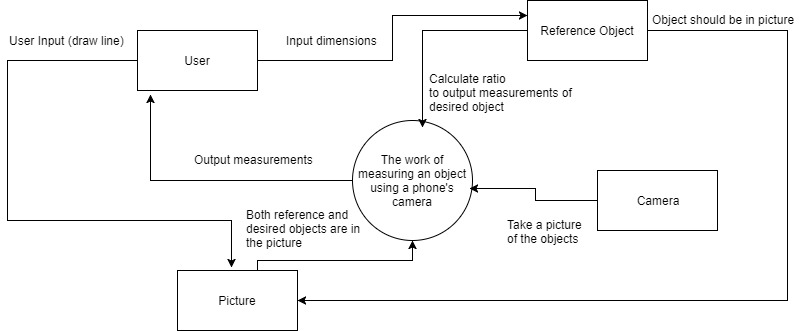
\includegraphics[width=6in]{work.jpg} 
   \caption{Work Context Diagram}
   \label{fig:1}
\end{figure}

\subsubsection{Work Partitioning}
	\begin{table}[H]

	\begin{tabular}{|c|c|L|}
		\hline
		\hline
		Event Name & Input/Output & Summary\\
		\hline
		User Takes Picture & Picture(IN) & The user takes a picture of the object and the application prepares the pic to be analyzed for length measurement\\
		\hline
		User selects object and reference object& Lines on the objects(IN) & The user draws on the line on the objects for the application to do calculation \\ 
		\hline 
		User inputs the reference objects length & 
		Reference Object length (IN) & The user inputs the reference object's length in the picture in cm, meters, or inches in order to calculate actual object's length \\
		\hline
		Application does calculation & Length(OUT) & The application uses all the information given by the user to output the objects length \\ 
		\hline
		\hline
	\end{tabular}
		\caption{\textcolor{red}{Work Partitioning}}
		\label{table:2}
\end{table}

\subsubsection{Individual Product Use Cases}
\begin{figure}[H]
   \centering
   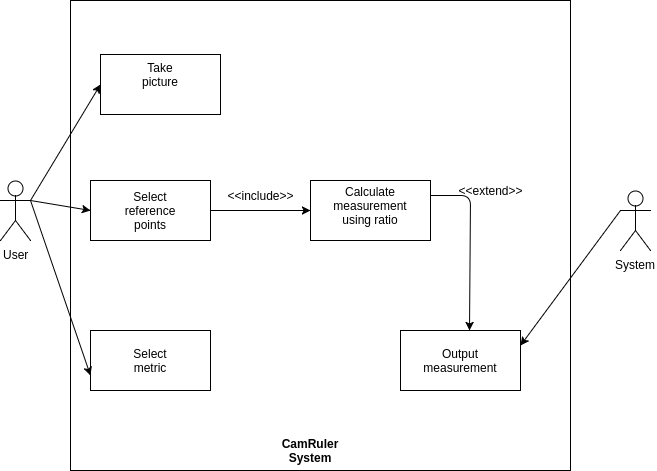
\includegraphics[width=6in]{use_cases.png} 
   \caption{Use Cases Diagram}
   \label{fig:2}
\end{figure}
\subsection{Functional Requirements}
\begin{enumerate}{}{}
\item FR1 \\Description: The executable android application will open an graphical user interface on android phone. \\ \\
 Test Case: Check to see if the GUI opens upon executing the application 

\item FR2 \\Description: The android application displays instructions for the use of the application in and waits for user input \\ \\
 Test Case: Check if application does what the instructions say

<<<<<<< HEAD
<<<<<<< HEAD
\item FR3 \\Description: Upon the reception of user input the application opens the phone’s camera application for the user to take a picture of the reference object(an object with it’s length known) and the objects to be measured, all together in the same picture.\sout{ Otherwise if the camera application fails, it allows the user to pick a picture from the phone's gallery} \\ \\
 Test Case: Check to see if the camera opens up to take a picture

\item FR4 \\Description: After the picture is taken, it is set to the specified image area in the application.  The application then allows the User to draw  two dots or four dots, each one at the ends of the reference object on the picture as well as the object to be measured. \\\\
 Test Case: Check to see if one can draw properly on the picture and if a line is created\\ 
  Check to see if the picture becomes the background of the application

\item FR5\\Description: After the 2nd dot of each object is drawn, a line is shown from one point to the other. The user can no longer draw after the line is shown. \\ \\
=======
=======
>>>>>>> b3d29f909f0c5e968073f1f1c5d72866dcf5a07a
\item FR3 \\Description: Upon the reception of user input the application opens the phone’s camera application for the user to take a picture of the reference object(an object with it’s length known) and the object to be measured, all together in the same picture. Otherwise if the camera application fails, it allows the user to pick a picture from the phone's gallery \\ \\
 Test Case: Check to see if the camera opens up to take a picture

\item FR4 \\Description: After the picture is taken, it is set to the specified image area in the application.  The application then allows the User to draw  two dots, each one at the ends of the reference object on the picture as well as the object to be measured. \\\\
 Test Case: Check to see if one can draw properly on the picture and if a line is created\\ 
  Check to see if the picture becomes the background of the application

\item FR5\\Description: After the 2nd dot is drawn, a line is shown from one point to the other. The user can no longer draw after the line is shown. \\ \\
<<<<<<< HEAD
>>>>>>> b3d29f909f0c5e968073f1f1c5d72866dcf5a07a
=======
>>>>>>> b3d29f909f0c5e968073f1f1c5d72866dcf5a07a
 Test Case: Line from 1st dot to 2nd dot after the 2nd dot is drawn \\ \\
  Check to see what happens if drawing is still possible after the line is shown

\item FR6 \\Description:The user has an option to retake picture and re-select their points on the picture \\   \\          
 Test Case: Take two pics from the same state and redraw points after drawn once  from the same state

\item FR7 \\Description: After the lines are drawn, the application opens a dialog box for the user to input the measurements of the reference object \\ \\
 Test Case: Check to see if the dialog box opens\\
  Check to see if the dialog box allows the user to input measurements in different units (cm, m, inches)

\item FR8 \\Description: After the the two lines are shown, the application calculates the length of the object and displays the length in cm, meters, and inches. \\	  \\
 Test Case: test if the calculation is correct my measuring the actual object \\
<<<<<<< HEAD
<<<<<<< HEAD
 
 {\color{red}\item FR9 \\Description: When placing the points on the picture, the user is able to drag the points. \\	  \\
 Test Case: Check if you can drag each point when placing on picture }\\

 
=======

>>>>>>> b3d29f909f0c5e968073f1f1c5d72866dcf5a07a
=======

>>>>>>> b3d29f909f0c5e968073f1f1c5d72866dcf5a07a
\end{enumerate}
\section{Non-functional Requirements}

\subsection{Look and Feel Requirements}
\subsubsection{Appearance Requirements}
NF-AP \\
<<<<<<< HEAD
<<<<<<< HEAD
The product shall display the logo as the application icon. CamRuler’s background will also contain the logo until a picture is taken to fill the background. \sout{It will have a slick green theme that all the buttons and message windows will follow}
{\color{red}Fit Criterion: Ask 10 people to rate the looks of the app and  75 percent of the people should rate it over 5 }
=======
The product shall display the logo as the application icon. CamRuler’s background will also contain the logo until a picture is taken to fill the background. It will have a slick green theme that all the buttons and message windows will follow

>>>>>>> b3d29f909f0c5e968073f1f1c5d72866dcf5a07a
=======
The product shall display the logo as the application icon. CamRuler’s background will also contain the logo until a picture is taken to fill the background. It will have a slick green theme that all the buttons and message windows will follow

>>>>>>> b3d29f909f0c5e968073f1f1c5d72866dcf5a07a

\subsection{Usability and Humanity Requirements}
\subsubsection{Ease of Use Requirements}
NF-EU\\
The product shall make it easy to select objects in the picture and provide a satisfactory experience for any user using this product.
<<<<<<< HEAD
<<<<<<< HEAD
{\color{red}Fit Criterion: Ask 10 people to rate the looks of the app and  75 percent of the people should rate it over 5 }
=======
>>>>>>> b3d29f909f0c5e968073f1f1c5d72866dcf5a07a
=======
>>>>>>> b3d29f909f0c5e968073f1f1c5d72866dcf5a07a

\subsubsection{Understandability and Politeness Requirements}
NF-UPR\\
The product shall use metrics familiar with the user and hide the details of length calculation from the user 
<<<<<<< HEAD
<<<<<<< HEAD
{\color{red}Fit Criterion: Ask 10 people to rate the metrics familiarity of the app and  75 percent of the people should rate it over 5 }

\subsubsection{Learning Requirements}
NF-LR \\
The user must have some knowledge of operating a phone 
{\color{red}Fit Criterion: User should have some experience with a phone}
=======
=======
>>>>>>> b3d29f909f0c5e968073f1f1c5d72866dcf5a07a

\subsubsection{Learning Requirements}
NF-LR \\
The user must have some of operating a phone 
<<<<<<< HEAD
>>>>>>> b3d29f909f0c5e968073f1f1c5d72866dcf5a07a
=======
>>>>>>> b3d29f909f0c5e968073f1f1c5d72866dcf5a07a

\subsubsection{Accessibility Requirements}
NF-AR \\
The android application will be executed by different models of android phones
<<<<<<< HEAD
<<<<<<< HEAD
{\color{red}Fit Criterion: The android application should run with no errors on 5 different models }
=======
>>>>>>> b3d29f909f0c5e968073f1f1c5d72866dcf5a07a
=======
>>>>>>> b3d29f909f0c5e968073f1f1c5d72866dcf5a07a


\subsection{Performance Requirements}
\subsubsection{Speed and Latency Requirements}
NF-SLR \\
<<<<<<< HEAD
<<<<<<< HEAD
The application shall respond almost immediately upon user input and during calculation of length.
{\color{red}Fit Criterion: The application should respond with in 1 second upon user input and calculation  }
=======
The application shall respond almost immediately upon user input and during calculation of length 
>>>>>>> b3d29f909f0c5e968073f1f1c5d72866dcf5a07a
=======
The application shall respond almost immediately upon user input and during calculation of length 
>>>>>>> b3d29f909f0c5e968073f1f1c5d72866dcf5a07a

\subsubsection{Safety-Critical Requirements}
NF-SCR \\
The product shall not compromise phone or the picture the user takes
<<<<<<< HEAD
<<<<<<< HEAD
{\color{red}Fit Criterion: The product shall not compromise data used from the phone }
=======
>>>>>>> b3d29f909f0c5e968073f1f1c5d72866dcf5a07a
=======
>>>>>>> b3d29f909f0c5e968073f1f1c5d72866dcf5a07a

\subsubsection{Precision or Accuracy Requirements}
NF-PAR \\
Output of length will be accurate to 3 decimal places
<<<<<<< HEAD
<<<<<<< HEAD
{\color{red}Fit Criterion: The output shall be accurate to 3 decimal places }
=======
>>>>>>> b3d29f909f0c5e968073f1f1c5d72866dcf5a07a
=======
>>>>>>> b3d29f909f0c5e968073f1f1c5d72866dcf5a07a

\subsubsection{Reliability and Availability Requirements}
NF-RAR \\
The product shall be available on the user’s phone once the user downloads the application 
<<<<<<< HEAD
<<<<<<< HEAD
{\color{red}Fit Criterion: 100 percent of users that download the app shall have the product available on the user's phone}

\subsubsection{Robustness or Fault-Tolerance Requirement}
NF-RFTR \\
The product shall work without access to internet
{\color{red}Fit Criterion: The product shall work 100 percent of the time wihtout access to internet }

\subsubsection{Capacity Requirements}
NF-CR \\
{\color{red}The product shall be able to measure multiple objects from the taken picture }
{\color{red}Fit Criterion: The product shall be able to measure 1 or 2 objects from the taken picture }
=======
=======
>>>>>>> b3d29f909f0c5e968073f1f1c5d72866dcf5a07a

\subsubsection{Robustness or Fault-Tolerance Requirement}
NF-RFTR \\
The product shall work without access to internet and the product shall be able to select a picture from gallery if camera does not work

\subsubsection{Capacity Requirements}
NF-CR \\
The product shall be able to measure exactly one object in a picture 
<<<<<<< HEAD
>>>>>>> b3d29f909f0c5e968073f1f1c5d72866dcf5a07a
=======
>>>>>>> b3d29f909f0c5e968073f1f1c5d72866dcf5a07a

\subsubsection{Scalability or Extensibility Requirements}
NF-SER \\
The product shall be capable of measuring multiple objects in one picture after a few days of launch
<<<<<<< HEAD
<<<<<<< HEAD
{\color{red}Fit Criterion:The product shall be able to measure 2 to 3 object after a fewdays of launch }
=======
>>>>>>> b3d29f909f0c5e968073f1f1c5d72866dcf5a07a
=======
>>>>>>> b3d29f909f0c5e968073f1f1c5d72866dcf5a07a

\subsubsection{Longevity Requirements}
NF-LR \\
The product shall be relevant for the lifetime of android phones
<<<<<<< HEAD
<<<<<<< HEAD
{\color{red}Fit Criterion: The product shall be relevant for 20years  }
=======
>>>>>>> b3d29f909f0c5e968073f1f1c5d72866dcf5a07a
=======
>>>>>>> b3d29f909f0c5e968073f1f1c5d72866dcf5a07a


\subsection{Operational and Environmental Requirements}

\subsubsection{Expected Physical Environment}
NF-EPE \\
The product shall be usable in an environment where a phone is acceptable 
<<<<<<< HEAD
<<<<<<< HEAD
{\color{red}Fit Criterion: The product shall be usable indoors and outdoors in a non-wet environment}
=======
>>>>>>> b3d29f909f0c5e968073f1f1c5d72866dcf5a07a
=======
>>>>>>> b3d29f909f0c5e968073f1f1c5d72866dcf5a07a

\subsubsection{Requirements for Interfacing with Adjacent Systems}
NF-RIA \\
The production shall work on recent versions of android
<<<<<<< HEAD
<<<<<<< HEAD
{\color{red}Fit Criterion: The product shall work on android 4.0 and up }

 \subsubsection{Productization Requirements}
 NF-PR \\
The product shall be distributed as an android application 
{\color{red}Fit Criterion: The product shall be able to distribute on a phone running an android operating system }
=======
=======
>>>>>>> b3d29f909f0c5e968073f1f1c5d72866dcf5a07a

 \subsubsection{Productization Requirements}
 NF-PR \\
The product shall be distributed as a android application 
<<<<<<< HEAD
>>>>>>> b3d29f909f0c5e968073f1f1c5d72866dcf5a07a
=======
>>>>>>> b3d29f909f0c5e968073f1f1c5d72866dcf5a07a

\subsubsection{Release Requirements}
NF-RR \\
The product will undergo maintenance upon realization of any errors in calculation or user interface
<<<<<<< HEAD
<<<<<<< HEAD
{\color{red}Fit Criterion: The product will undergo maintentance after realizing 1 or more errors}
=======
>>>>>>> b3d29f909f0c5e968073f1f1c5d72866dcf5a07a
=======
>>>>>>> b3d29f909f0c5e968073f1f1c5d72866dcf5a07a




\subsection{Maintainability and Support Requirements}
\subsubsection{Maintenance Requirement}
NF-MR \\
Minimal product maintenance 
<<<<<<< HEAD
<<<<<<< HEAD
{\color{red}Fit Criterion: The product shall require maintenance once a year }
=======
>>>>>>> b3d29f909f0c5e968073f1f1c5d72866dcf5a07a
=======
>>>>>>> b3d29f909f0c5e968073f1f1c5d72866dcf5a07a

\subsubsection{Supportability Requirements}
NF-SR \\
Ensure that most  android users can use the app
<<<<<<< HEAD
<<<<<<< HEAD
{\color{red}Fit Criterion: Ask 10 people if they can use the app and 90 percent of the people should be able to use it }

\subsubsection{Adaptability Requirement}
NF-AR \\
The app shall be universally accessible by users
{\color{red}Fit Criterion: The app should be accessible in all counties with access to internet}
=======
=======
>>>>>>> b3d29f909f0c5e968073f1f1c5d72866dcf5a07a

\subsubsection{Adaptability Requirement}
NF-AR \\
The app shall be universally accessible by users 
<<<<<<< HEAD
>>>>>>> b3d29f909f0c5e968073f1f1c5d72866dcf5a07a
=======
>>>>>>> b3d29f909f0c5e968073f1f1c5d72866dcf5a07a

\subsection{Security Requirements}
\subsubsection{Access Requirement}
NF-SAR \\
The entire general public shall be able to access the game assuming they have internet to download the app 
<<<<<<< HEAD
<<<<<<< HEAD
{\color{red}Fit Criterion: 100 percent of people with access to the internet shall be able to download the app}

\subsubsection{Integrity Requirement}
NF-SIR \\
The app shall not allow the user to put invalid input
{\color{red}Fit Criterion: The app should allow 0 invalid input }
\subsubsection{Privacy Requirement}
NF-SPR \\
The product shall not save any picture the user takes
{\color{red}Fit Criterion: The product shall save 0 picture the user takes}
=======
=======
>>>>>>> b3d29f909f0c5e968073f1f1c5d72866dcf5a07a

\subsubsection{Integrity Requirement}
NF-SIR \\
The app shall not all the user to put invalid input

\subsubsection{Privacy Requirement}
NF-SPR \\
The product shall not save any picture the user takes
<<<<<<< HEAD
>>>>>>> b3d29f909f0c5e968073f1f1c5d72866dcf5a07a
=======
>>>>>>> b3d29f909f0c5e968073f1f1c5d72866dcf5a07a

\subsection{Cultural Requirements}
NF-SCR \\
The product shall offer output in multiple  types of metric unit
<<<<<<< HEAD
<<<<<<< HEAD
{\color{red}Fit Criterion: The product shall offer output in 4 different metric types }
=======
>>>>>>> b3d29f909f0c5e968073f1f1c5d72866dcf5a07a
=======
>>>>>>> b3d29f909f0c5e968073f1f1c5d72866dcf5a07a

\subsection{Legal Requirements}
\subsubsection{Compliance Requirements}
NF-LCR \\
<<<<<<< HEAD
<<<<<<< HEAD
The app shall not compromise any laws
{\color{red}Fit Criterion: The app shall break 0 laws }
=======
The app shall not compromise any laws 
>>>>>>> b3d29f909f0c5e968073f1f1c5d72866dcf5a07a
=======
The app shall not compromise any laws 
>>>>>>> b3d29f909f0c5e968073f1f1c5d72866dcf5a07a

\subsubsection{Standards Requirements}
NF-LSR \\
The app shall adhere to the GNU general public license 
<<<<<<< HEAD
<<<<<<< HEAD
{\color{red}Fit Criterion: The app shall adhere to the GNU general public license }
=======
>>>>>>> b3d29f909f0c5e968073f1f1c5d72866dcf5a07a
=======
>>>>>>> b3d29f909f0c5e968073f1f1c5d72866dcf5a07a

\subsection{Health and Safety Requirements}
NF-LHSR \\
not applicable 

\section{Project Issues}

\subsection{Open Issues}
We still need to investigate how to use Android Studio as we have little experience with it. Other open issues will be added after we have begun developing our implementation.

\subsection{Off-the-Shelf Solutions}
\subsubsection{Ready-Made Products}
\begin{itemize}
\item Camera Ruler Beta Version Android Application
    \item{Application works, but is still being further developed before being released to general public on app store}
\end{itemize}

\subsubsection{Reusable Components}
\begin{itemize}
    \item Development not yet started, so reusable components not yet recognized (if available).
\end{itemize}

\subsubsection{Products That Can Be Copied}
\begin{itemize}
\item Can use interface and organization of Camera Ruler Beta Application
\end{itemize}

\subsection{New Problems}
\subsubsection{Effects on the Current Environment}
Adding in the feature to enable users to zoom into pictures for a more precise selection of the reference point may cause some errors which we will need to account for as the code right now does not account for zooming into the picture. If no additional features are added, no effects on the current environment are foreseen.

\subsubsection{Effects on the Installed Systems}
Recreating an Android application to work on Android devices should cause no errors. Also, this interface is planned to stand alone and hence, will not impact any other systems.

\subsubsection{Potential User Problems}
Prior to implementation, a potential user problem we think may occur is not being able to click the correct spot and hence, getting a slightly inaccurate measurement. Users will be warned that the measurement is only as accurate as they tap on the correct spot. However, as developers, we plan to try and create a zoom feature which will enable the user to be more accurate in point selection. 

\subsubsection{Limitations in the Anticipated Implementation Environment That May Inhibit the New Product}
Being an already existing application that works in beta form, we know that our application, if done correctly and as planned, should work on Android devices. Only limitation is doing the application on Android Studio may be tough as there is a time constraint of approximately 2.5 months.
\subsection{Tasks}
Tasks for this project have been outlined by the course instructor of Software Engineering 3XA3. Deliverables include the Problem Statement, Proof of Concept plan, Requirements document revision 0, Test plan revision 0, Proof of concept demonstration, Design document revision 0, Revision 0 demonstration, Peer evaluation of other teams revision 0, User’s guide revision 0, Test report revision 0, Final demonstration (Revision 1), and Final documentation (Revision 1).  The final project is due on December 6th, 2017. Our project plan is created on a Gantt chart which is available on gitlab. Use of the waterfall method will be used to get our project successfully completed. However, the main thing is that we need to stay on top of time constraints as that is our only worry.
\subsection{Migration to the New Product}
\subsubsection{Requirements for Migration to the New Product}
We may need to find similar libraries to which Camera Ruler used to stay consistent with requirements which would work with Android Studio as well. However, we are still planning our implementation so this may change and we may not need similar libraries to the parent application.

\subsubsection{Data That Has to Be Modified or Translated for the New System}
No data needs to be translated for the new system, however, to be safe, we will verify the mathematical calculations provided by Camera Ruler to be safe. This verification is planned to take place right before the implementation of the application and will be done by ratio calculations. 
\subsection{Risks}
Risks we found were related to the development of the product. It may be too complex for us as we are still learning Android Studio and making an Android Application. After having this completed, we also need to make sure it works properly where testing may also be complicated as there are multiple aspects to test such as if the picture taken is the background of the app, and if reference points are able to be placed and dragged to the correct spot. All in all, schedule pressure seems to be the only risk at the moment.

\subsection{Costs}
No money is going into the making of this application, but the cost we may have would be related to time as we may not get enough time to implement all that we have planned to implement at the moment. 

\subsection{User Documentation and Training}
\subsubsection{User Documentation Requirements}
Instructions on how to use the application will follow in sequence on the application. With our planned interface being very simple, the user will be prompted to take a picture they want to measure along with a reference object in the same picture and then will be asked to pick points to measure in the metric they have selected. Due to this simplicity, we do not plan on creating a separate user manual/help guide, as the instructions will be on screen for the user to follow.

\subsubsection{Training Requirements}
As aforementioned, the simplicity of this application is such that no training will be required for the user.

\subsection{Waiting Room}
<<<<<<< HEAD
<<<<<<< HEAD
A new feature which could be added would be \sout{dragging the reference points so that more accurate measurements could be made. To do this, more research will be done on dragging and dropping on a live interface. Another idea} to have more accurate measurements would be to zoom into a picture so the exact point of measurement could be determined. As of now we only have measurements in straight lines, so a future implementation could be to allow users to measure objects in curved shapes as well. 

\subsection{Ideas for Solutions}
For zooming into a picture, \sout{dragging points}, or measuring curved objects we do not have any ideas, so more research and planning will need to be done in order to actually implement these ideas. 
=======
=======
>>>>>>> b3d29f909f0c5e968073f1f1c5d72866dcf5a07a
A new feature which could be added would be dragging the reference points so that more accurate measurements could be made. To do this, more research will be done on dragging and dropping on a live interface. Another idea to have more accurate measurements would be to zoom into a picture so the exact point of measurement could be determined. As of now we only have measurements in straight lines, so a future implementation could be to allow users to measure objects in curved shapes as well. 

\subsection{Ideas for Solutions}
For zooming into a picture, dragging points, or measuring curved objects we do not have any ideas, so more research and planning will need to be done in order to actually implement these ideas. 
<<<<<<< HEAD
>>>>>>> b3d29f909f0c5e968073f1f1c5d72866dcf5a07a
=======
>>>>>>> b3d29f909f0c5e968073f1f1c5d72866dcf5a07a


\end{document}

